\begin{tikzpicture}
\tikzset{
    overlay box/.style={fill=white,fill opacity=0.9}
}
\node[overlay,anchor=north west,inner sep=0mm] (base) at (0, 0) {
    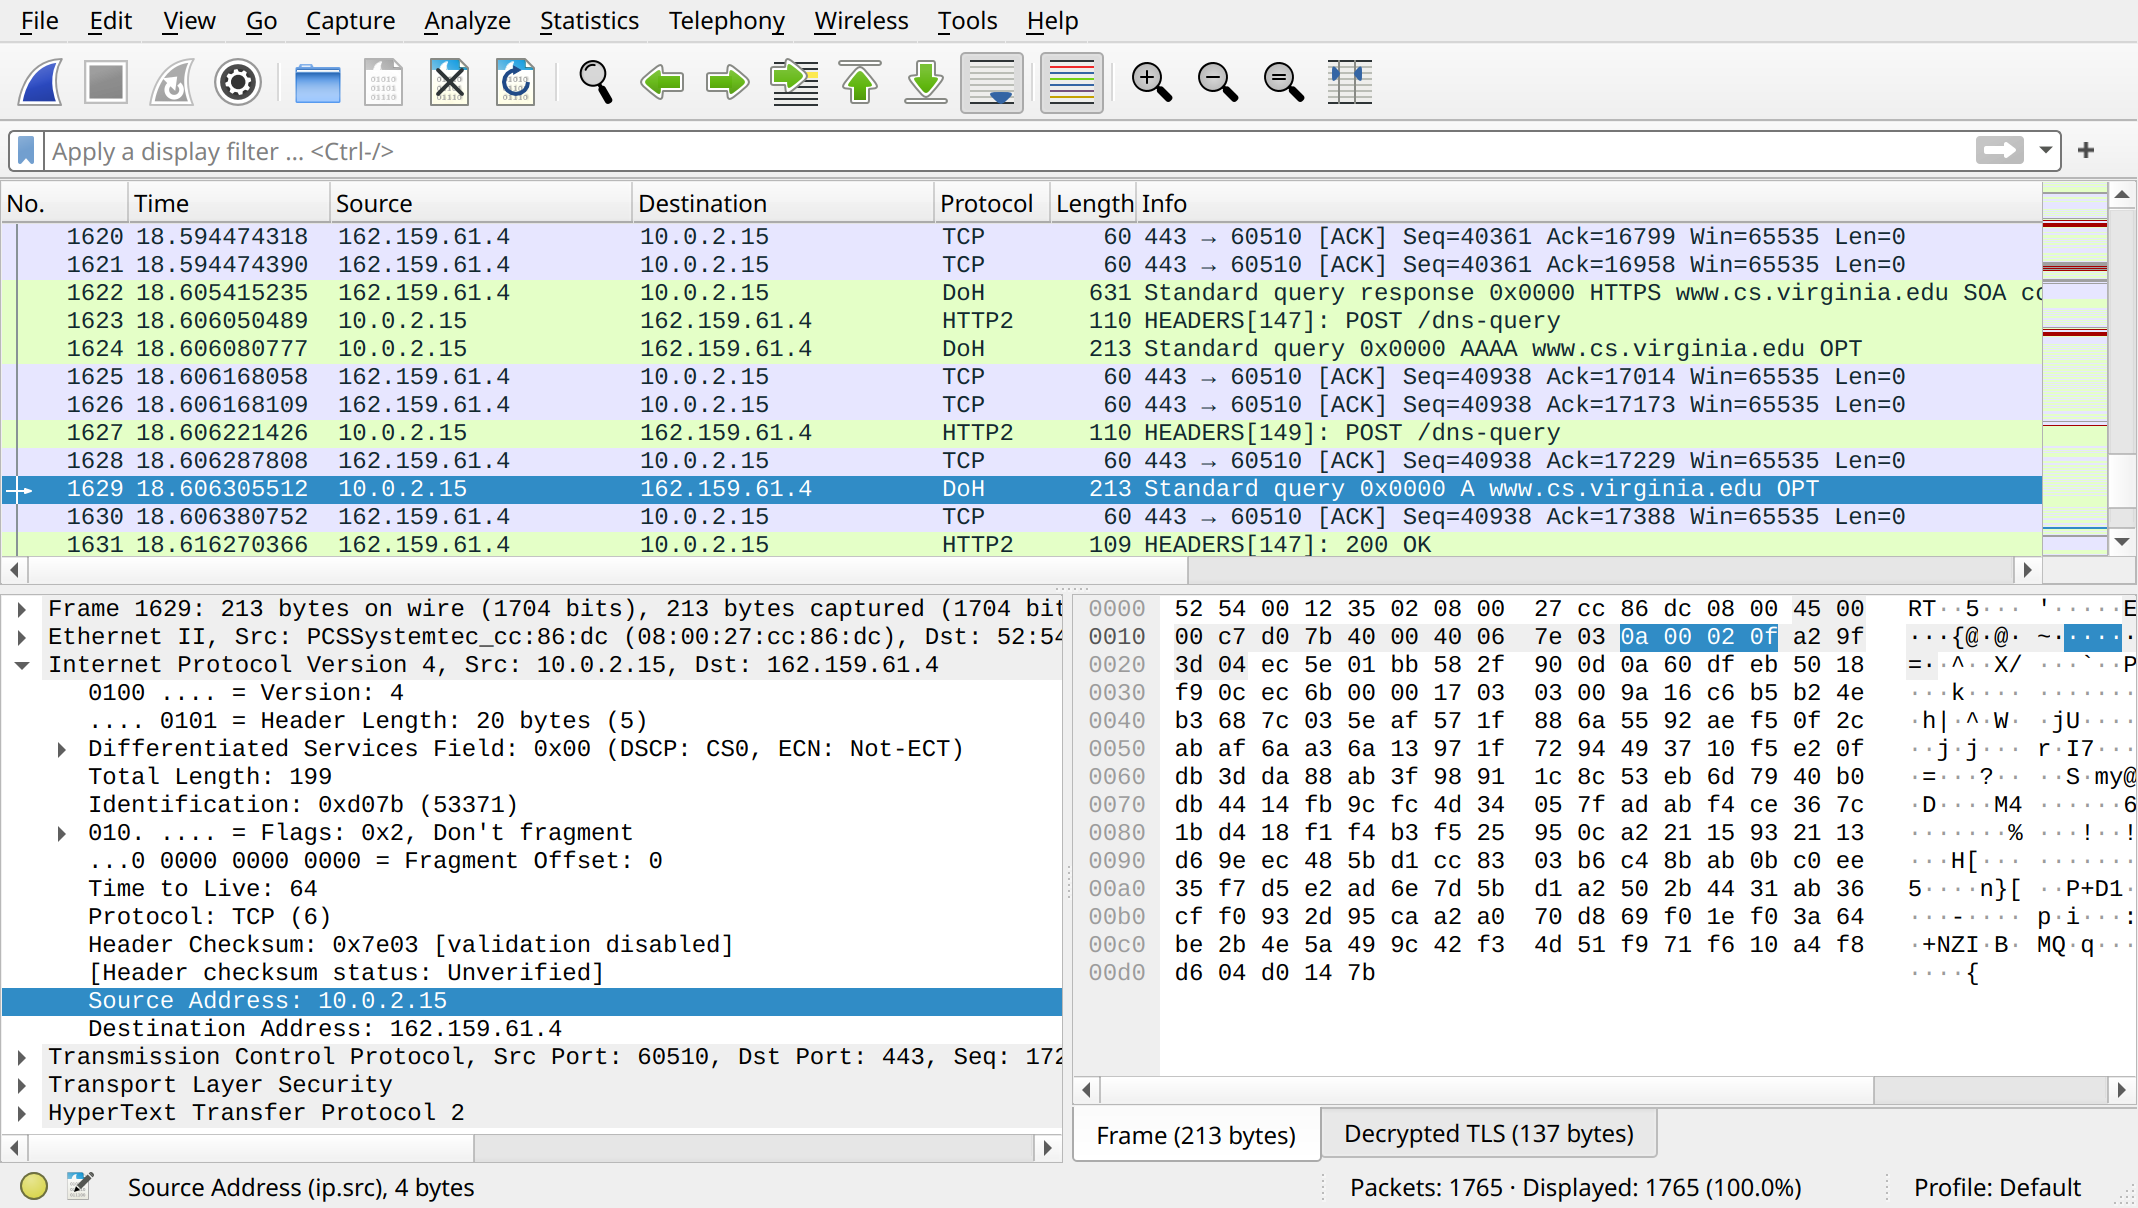
\includegraphics[width=\mypaperwidth]{../intro/wireshark-example1.png}
};
\begin{visibleenv}<1>
    \node[text=red,overlay box] at (7.5, -2) {wireshark window};
\end{visibleenv}
\path (0, 0) rectangle (14.5, -7); % for bounding box
%\draw[overlay,help lines] (0, 0) grid (14, -8);
\begin{visibleenv}<3>
    \path[draw,red,very thick] (0, -1.2) rectangle (14.5, -4)
        node[midway,overlay box] { packet list };
    \path[draw,red,very thick] (0, -4) rectangle (7.25, -7.9)
        node[midway,overlay box] { packet details };
    \path[draw,red,very thick] (7.25, -4) rectangle (14.5, -7.9)
        node[midway,overlay box] { packet bytes };
\end{visibleenv}
\begin{visibleenv}<4>
    \path[draw,red,very thick] (0, -6.7) rectangle (7.2, -6.9);
    \path[draw,red,very thick] (10.93, -4.2) rectangle (12.1, -4.4);
    \path[draw,red,ultra thick] (7.2, -6.8) -- (10.93, -4.3)
        node[midway,above left,overlay box,align=left] {
            hilite in details \\
            shows corresponding bytes
        }
        node[midway,below right,overlay box,font=\fontsize{10}{11}\selectfont,text=black,align=left] {
            this case: \\
            \texttt{10} = \texttt{0x0a} \\
            \texttt{0} = \texttt{0x00} \\
            \texttt{2} = \texttt{0x02} \\
            \texttt{15} = \texttt{0x0f}
        };
\end{visibleenv}
\begin{visibleenv}<5>
    \path[draw,red,very thick] (6.3, -1.2) rectangle (7.15, -4);
    \node[overlay box,anchor=west] at (7.15, -3) (protocol) {`protocol'};
    \node[overlay box,font=\small,anchor=north west] at (protocol.south west) {
        the highest-layer protocol decoded
    };
\end{visibleenv}
\begin{visibleenv}<6-7>
    \begin{scope}
        \begin{pgfinterruptboundingbox}
    \tikzset{invclip/.style={clip,insert path={{[reset cm]
          (-16383.99999pt,-16383.99999pt) rectangle (16383.99999pt,16383.99999pt)
      }}}}
        \path[invclip] (6.3, -3.2) rectangle (7.15, -3.4);
        \end{pgfinterruptboundingbox}

        \fill[overlay,white,fill opacity=0.8] (0, 0) rectangle (14.5, -1.2);
        \fill[white,fill opacity=0.8] (0, -1.2) rectangle (14.5, -4);
        \fill[white,fill opacity=0.8] (7.25, -4) rectangle (14.5, -7.9);
    \end{scope}
    \path[draw,red,very thick] (0, -4) rectangle (7.25, -7.9);
    \tikzset{
        protomark/.style={Latex-,blue,thick},
        protomark brace/.style={blue,thick,decorate,decoration={brace}},
        protomark label/.style={blue,fill=white,fill opacity=0.9},
    }
    \draw[protomark] (7.25, -4.3) -- ++(1, 0) node[right,protomark label] {ethernet};
    \draw[protomark brace] (7.3, -4.5) -- (7.3, -7.1);
        \draw[protomark] (7.4, -5.8) -- ++ (0.75, .6) node[right, protomark label] {
                IPv4 (internet protocol version 4)
        };
    \draw[protomark] (7.25, -7.2) -- ++(1, 1) node[right,protomark label] {
        TCP ({\fontsize{10}{11}\selectfont transmission control protocol})
    };
    \draw[protomark] (7.25, -7.325) -- ++(1, .5) node[right,protomark label] {
        TLS ({\fontsize{10}{11}\selectfont transport layer security})
    };
    \draw[protomark] (7.25, -7.45) -- ++(1, -.2) node[right,protomark label] {
        HTTP/2 ({\fontsize{10}{11}\selectfont hypertext transfer protocol 2})
    };
\end{visibleenv}
\begin{visibleenv}<7>
    \draw[red, very thick] (6.3, -3.2) rectangle (7.15, -3.4);
    \draw[red,Latex-,very thick] (7.15, -3.3) -- ++(1, 0) node[right,align=left,overlay box] {
        DoH is not \\one of these!
    };
\end{visibleenv}
\end{tikzpicture}